\documentclass{minimal}
\usepackage[T1]{fontenc}
\usepackage{newtxtext}
\usepackage{newtxmath}
\usepackage{tikz}
\usetikzlibrary{arrows.meta,calc,positioning}

\pdfpagewidth=1000pt
\pdfpageheight=360pt
\setlength{\paperwidth}{1000pt}
\setlength{\paperheight}{360pt}
\setlength{\textwidth}{1000pt}
\setlength{\textheight}{360pt}
\setlength{\oddsidemargin}{-72pt}
\setlength{\topmargin}{-72pt}
\setlength{\headheight}{0pt}
\setlength{\headsep}{0pt}
\setlength{\footskip}{0pt}
\setlength{\parindent}{0pt}
\pagestyle{empty}

\begin{document}
\begin{tikzpicture}[x=1pt,y=1pt,font=\rmfamily,line cap=round,line join=round]
\tikzset{
  inference/.style={
    -{Latex[length=9pt,width=6pt]},
    draw=black,
    line width=2.2pt
  },
  training/.style={
    -{Latex[length=8pt,width=5pt]},
    draw=black!75,
    densely dashed,
    line width=1.8pt,
    preaction={draw=white,line width=5pt}
  },
  query/.style={
    -{Latex[length=7pt,width=5pt]},
    draw=black!58,
    densely dotted,
    line width=1.6pt
  },
  module/.style={
    rounded corners=8pt,
    draw=black,
    line width=1.55pt,
    fill=white,
    align=center,
    minimum height=48pt,
    inner sep=7pt
  },
  inputbox/.style={module,fill=black!4},
  contextbox/.style={module,fill=black!2},
  statebox/.style={module,fill=black!9},
  transitionbox/.style={module,fill=black!14,line width=2.0pt},
  outputbox/.style={module,fill=black!5},
  chip/.style={
    rounded corners=7pt,
    draw=black!72,
    line width=1.25pt,
    fill=white,
    align=center,
    minimum height=27pt,
    inner sep=5pt
  },
  trainbox/.style={
    rounded corners=6pt,
    draw=black!72,
    line width=1.3pt,
    fill=white,
    align=center,
    minimum height=34pt,
    inner sep=5pt
  },
  lossbox/.style={
    rounded corners=7pt,
    draw=black,
    line width=1.45pt,
    fill=black!7,
    align=center,
    minimum height=34pt,
    inner sep=5pt
  },
  testpanel/.style={
    rounded corners=9pt,
    draw=black!70,
    line width=1.35pt,
    fill=black!2
  },
  optionalpanel/.style={
    rounded corners=9pt,
    draw=black!48,
    densely dashed,
    line width=1.35pt,
    fill=black!7
  },
  testnode/.style={
    rounded corners=5pt,
    draw=black!68,
    line width=1.15pt,
    fill=white,
    align=center,
    minimum height=27pt,
    inner sep=4pt
  }
}

\useasboundingbox (0,0) rectangle (1000,360);
% Drawing body only. Expected canvas: (0,0)--(1000,360).
\fill[white] (0,0) rectangle (1000,360);

% Main inference field.
\draw[rounded corners=12pt,draw=black!22,line width=1.1pt,fill=black!1]
  (14,124) rectangle (986,346);

% Cloud-masked EO history with replaceable thumbnail slots.
\node[inputbox,minimum width=116pt,minimum height=82pt] (history) at (73,232) {};
\draw[draw=black!70,line width=1.1pt,fill=white]
  (38,244) rectangle (71,269);
\draw[draw=black!70,line width=1.1pt,fill=black!4]
  (49,248) rectangle (82,273);
\draw[draw=black!70,line width=1.1pt,fill=black!9]
  (60,252) rectangle (93,277);
\foreach \x in {68,76,84} {
  \draw[draw=black!55,line width=0.8pt] (\x,253) -- (\x,276);
}
\foreach \y in {259,267} {
  \draw[draw=black!55,line width=0.8pt] (61,\y) -- (92,\y);
}
\draw[draw=black!45,line width=1.0pt,densely dashed]
  (53,246) -- (80,272);
\node[align=center,text=black,font=\rmfamily\bfseries\fontsize{19}{22}\selectfont]
  at (73,216) {cloud-masked\\EO history};

% Context operator, projector, states, transition, closure, and prediction.
\node[contextbox,minimum width=136pt,minimum height=63pt,text width=124pt,
      font=\rmfamily\bfseries\fontsize{20}{23}\selectfont]
  (q) at (211,232) {history-only $q_\theta$\\[-1pt]
  \normalfont\fontsize{18}{21}\selectfont context operator};
\node[contextbox,minimum width=68pt,
      font=\rmfamily\bfseries\fontsize{20}{23}\selectfont]
  (proj) at (331,232) {$P_\rho$};

\node[statebox,minimum width=86pt,minimum height=70pt] (zt) at (420,232) {};
\draw[draw=black!72,line width=0.9pt,fill=white]
  (397,238) rectangle (443,266);
\foreach \x in {408.5,420,431.5} {
  \draw[draw=black!45,line width=0.65pt] (\x,238) -- (\x,266);
}
\foreach \y in {245,252,259} {
  \draw[draw=black!45,line width=0.65pt] (397,\y) -- (443,\y);
}
\node[font=\rmfamily\bfseries\fontsize{19}{22}\selectfont] at (420,215)
  {spatial $z_t$};

\node[transitionbox,minimum width=126pt,minimum height=65pt,
      font=\rmfamily\bfseries\fontsize{21}{24}\selectfont]
  (trans) at (560,232) {shared $T_\psi$};

\node[statebox,minimum width=90pt,minimum height=70pt] (zh) at (684,232) {};
\draw[draw=black!72,line width=0.9pt,fill=white]
  (660,238) rectangle (708,266);
\foreach \x in {672,684,696} {
  \draw[draw=black!45,line width=0.65pt] (\x,238) -- (\x,266);
}
\foreach \y in {245,252,259} {
  \draw[draw=black!45,line width=0.65pt] (660,\y) -- (708,\y);
}
\node[font=\rmfamily\bfseries\fontsize{19}{22}\selectfont] at (684,215)
  {$z_{t+h}$};

\node[outputbox,minimum width=84pt,minimum height=62pt,text width=74pt,
      font=\rmfamily\bfseries\fontsize{19}{22}\selectfont]
  (head) at (788,232) {state head\\$O_\omega$};
\node[circle,draw=black,line width=1.8pt,fill=white,minimum size=37pt,
      font=\rmfamily\bfseries\fontsize{23}{26}\selectfont]
  (plus) at (855,232) {$+$};
\node[outputbox,minimum width=112pt,minimum height=82pt] (pred) at (938,232) {};
\draw[draw=black!72,line width=1.0pt,fill=white]
  (911,246) rectangle (965,273);
\foreach \x in {924.5,938,951.5} {
  \draw[draw=black!45,line width=0.7pt] (\x,246) -- (\x,273);
}
\foreach \y in {255,264} {
  \draw[draw=black!45,line width=0.7pt] (911,\y) -- (965,\y);
}
\node[font=\rmfamily\bfseries\fontsize{19}{22}\selectfont] at (938,220)
  {forecast};
\node[font=\rmfamily\fontsize{19}{22}\selectfont] at (938,198)
  {$\widehat y_{t+h}$};

% Solid inference path.
\draw[inference] (history.east) -- (q.west);
\draw[inference] (q.east) -- (proj.west);
\draw[inference] (proj.east) -- (zt.west);
\draw[inference] (zt.east) -- (trans.west);
\draw[inference] (trans.east) -- (zh.west);
\draw[inference] (zh.east) -- (head.west);
\draw[inference] (head.east) -- (plus.west);
\node[text=black!70,font=\rmfamily\fontsize{18}{21}\selectfont]
  at (833,270) {$r_h$};
\draw[inference] (plus.east) -- (pred.west);

% History-only context inputs.
\node[chip,minimum width=90pt,
      font=\rmfamily\bfseries\fontsize{18}{21}\selectfont]
  (pastmet) at (169,311) {past met.};
\node[chip,minimum width=78pt,
      font=\rmfamily\bfseries\fontsize{18}{21}\selectfont]
  (qgeo) at (267,311) {static $g$};
\draw[inference,line width=1.45pt] (pastmet.south) -- ($(q.north)+(-24pt,0)$);
\draw[inference,line width=1.45pt] (qgeo.south) -- ($(q.north)+(24pt,0)$);

% Transition-only conditions.
\node[chip,minimum width=132pt,
      font=\rmfamily\bfseries\fontsize{18}{21}\selectfont]
  (weather) at (493,311) {full24 weather};
\node[chip,minimum width=78pt,
      font=\rmfamily\bfseries\fontsize{18}{21}\selectfont]
  (tgeo) at (617,311) {static $g$};
\node[chip,minimum width=94pt,
      font=\rmfamily\bfseries\fontsize{18}{21}\selectfont]
  (horizon) at (714,311) {horizon $h$};
\draw[inference,line width=1.45pt] (weather.south) -- ($(trans.north)+(-34pt,0)$);
\draw[inference,line width=1.45pt] (tgeo.south) -- (trans.north);
\draw[inference,line width=1.45pt] (horizon.south) -- ($(trans.north)+(34pt,0)$);

% Context-only prior is emitted before future weather enters.
\node[contextbox,minimum width=192pt,minimum height=46pt,
      font=\rmfamily\bfseries\fontsize{18}{21}\selectfont]
  (prior) at (407,153) {context-only prior $b_h$};
\draw[inference] ($(q.south)+(0,0)$) |- (prior.west);
\draw[inference] (prior.east) -- ++(244pt,0) |- (plus.south);

% Training-only band: every edge is dashed and separate from inference.
\draw[rounded corners=10pt,draw=black!55,densely dashed,line width=1.2pt,
      fill=black!2] (14,8) rectangle (986,111);
\node[anchor=west,text=black!72,
      font=\rmfamily\bfseries\fontsize{18}{21}\selectfont]
  at (27,98) {TRAINING ONLY};

% Future-state target branch.
\node[trainbox,minimum width=126pt,minimum height=48pt] (futureeo) at (97,53) {};
\draw[draw=black!65,line width=0.9pt,fill=white]
  (60,55) rectangle (83,73);
\draw[draw=black!65,line width=0.9pt,fill=black!7]
  (68,58) rectangle (91,76);
\node[font=\rmfamily\bfseries\fontsize{18}{21}\selectfont,
      align=center] at (111,52) {observed\\future EO};
\node[trainbox,minimum width=105pt,
      font=\rmfamily\bfseries\fontsize{18}{21}\selectfont]
  (frozenqp) at (241,53) {frozen $q+P$};
\node[statebox,minimum width=82pt,minimum height=43pt,
      font=\rmfamily\bfseries\fontsize{18}{21}\selectfont]
  (targetstate) at (357,53) {$z^\star_{t+20}$};
\node[lossbox,minimum width=187pt,minimum height=47pt,text width=174pt,
      font=\rmfamily\bfseries\fontsize{18}{21}\selectfont]
  (stateloss) at (512,53)
  {$\lambda_s\mathcal L_{\mathrm{future\text{-}state}}$\\[-1pt]
   \normalfont\fontsize{18}{21}\selectfont $h=20$ only};
\draw[training] (futureeo.east) -- (frozenqp.west);
\draw[training] (frozenqp.east) -- (targetstate.west);
\draw[training] (targetstate.east) -- (stateloss.west);
\draw[training] (zh.south) -- ++(0,-57pt) -| (stateloss.north);

% Output supervision: ground truth and frozen teacher never enter inference.
\node[trainbox,minimum width=126pt,
      font=\rmfamily\bfseries\fontsize{18}{21}\selectfont]
  (gt) at (696,35) {future target $y$};
\node[lossbox,minimum width=76pt,
      font=\rmfamily\bfseries\fontsize{18}{21}\selectfont]
  (gtloss) at (813,35) {$\mathcal L_{\mathrm{GT}}$};
\node[trainbox,minimum width=196pt,text width=184pt,
      font=\rmfamily\bfseries\fontsize{18}{21}\selectfont]
  (teacher) at (713,80) {frozen full-weather teacher};
\node[lossbox,minimum width=103pt,
      font=\rmfamily\bfseries\fontsize{18}{21}\selectfont]
  (kdloss) at (879,80) {$0.5\mathcal L_{\mathrm{KD}}$};
\draw[training] (gt.east) -- (gtloss.west);
\draw[training] (teacher.east) -- (kdloss.west);
\coordinate (predsupervision) at (953,110);
\draw[training] (pred.south) -- (predsupervision);
\draw[training] (predsupervision) |- (gtloss.east);
\draw[training] (predsupervision) |- (kdloss.east);

\end{tikzpicture}
\end{document}
